\chapter{Motion and Forces}

\section{Motion}

\begin{tcolorbox}[colback=red!5!white,colframe=red!75!black]
  \[\text{Average Speed}=\frac{\text{Distance}}{\text{Time}}\]
\end{tcolorbox}

If an object’s speed is changing throughout the distance measured, like a car speeding up as it gets on the highway, then this equation gives us its average speed during that time.

\vspace{.3cm}

\begin{figure}[htb!]
  \centering
  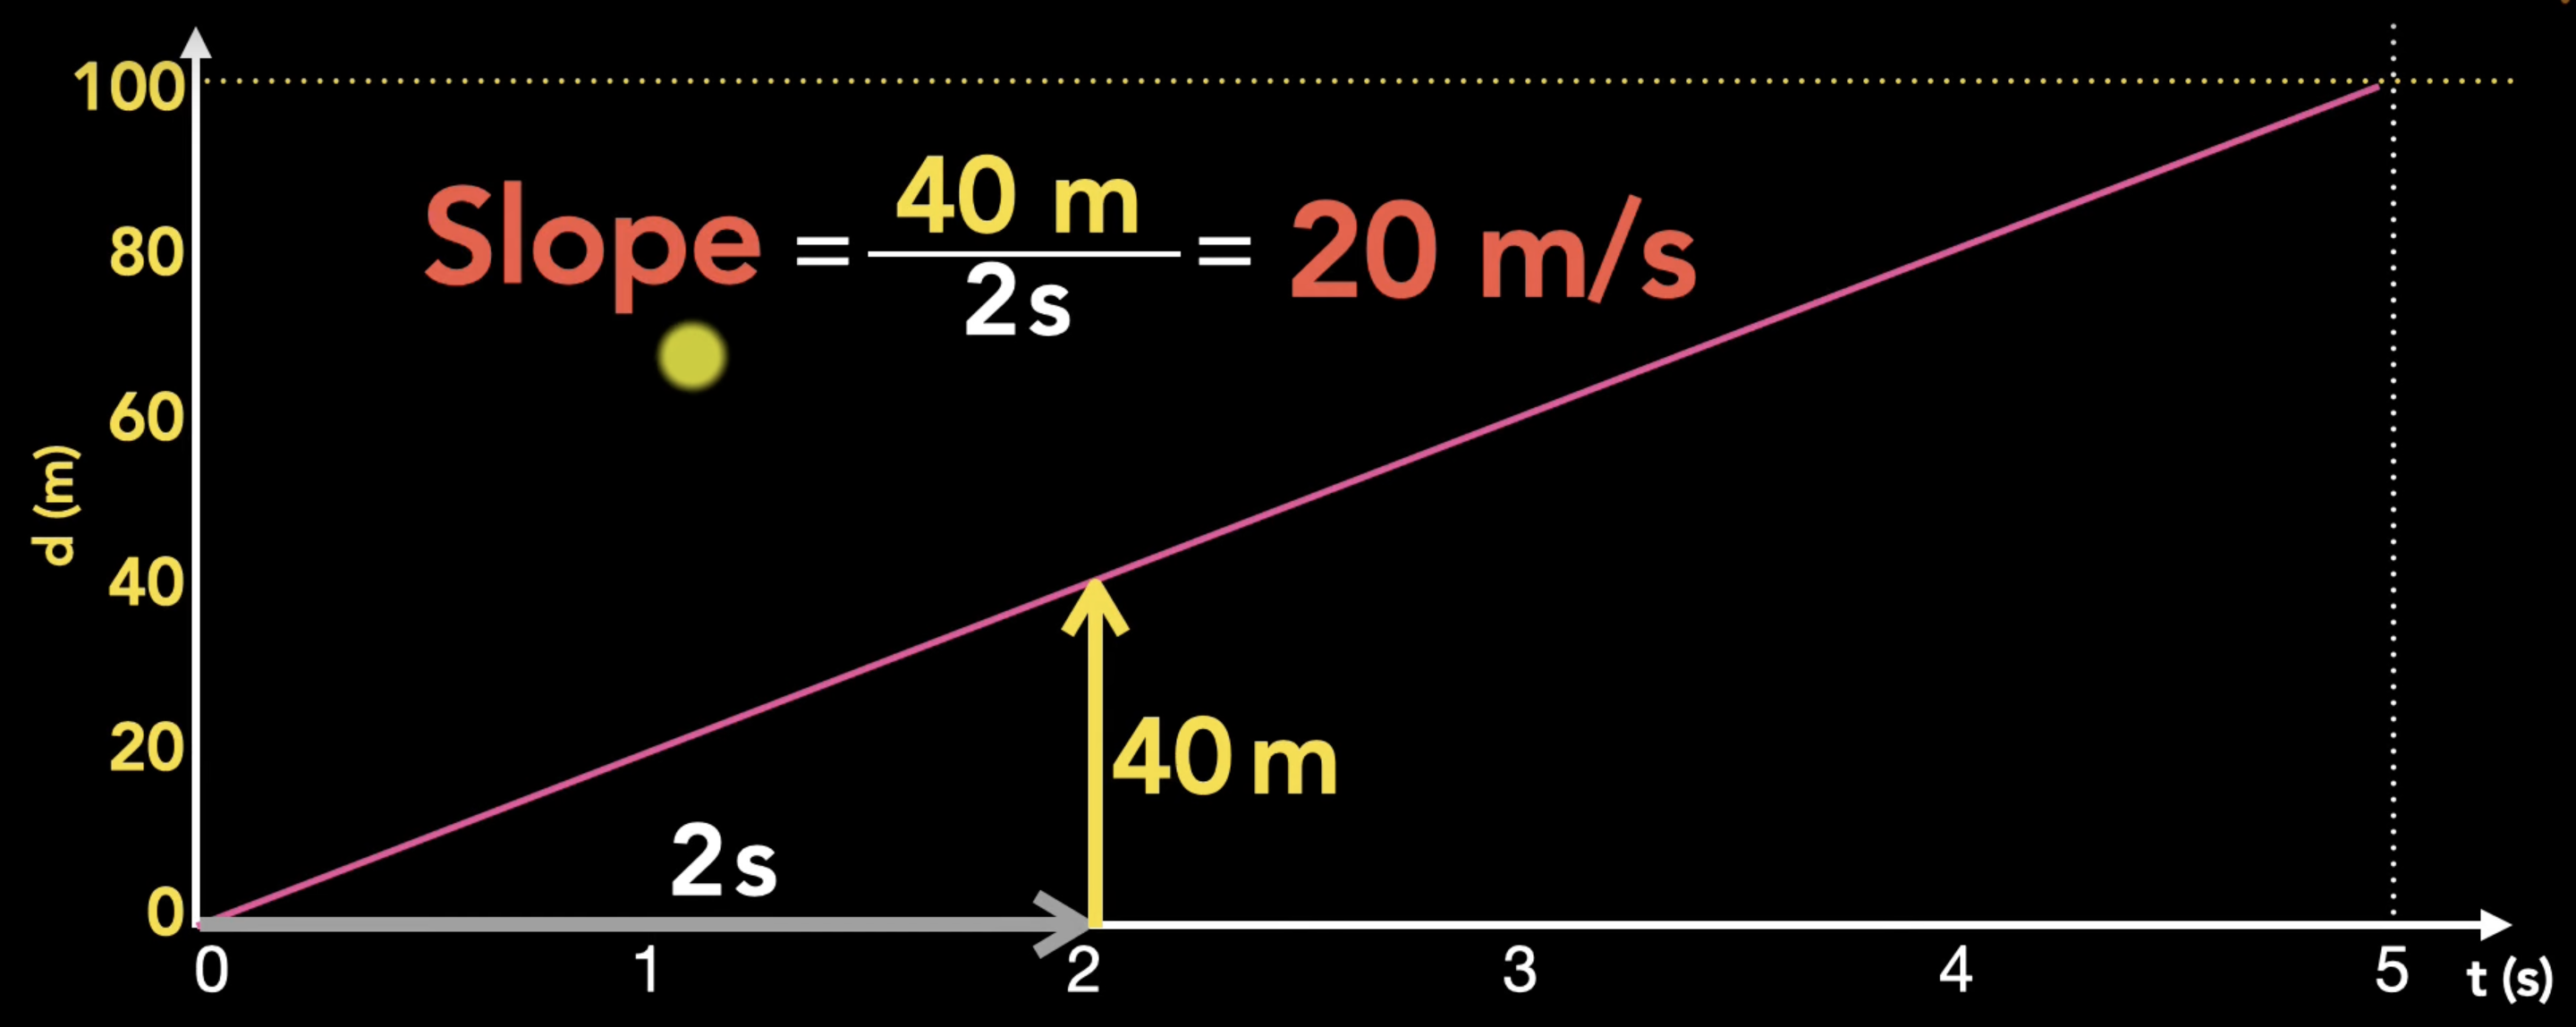
\includegraphics[width=0.8\textwidth]{0101.png}
  \caption{Graph of Speed}
\end{figure}

A \textbf{distance-time graph} shows the amount of time an object travels on the a-axis and the distance it travels in that time on the y-axis. The Speed of the object equals the \textbf{Slope} of the line.

\vspace{.5cm}

\hl{Velocity} (vận tốc) is speed plus direction. It measures how fast and in what direction an object moves.

% \vspace{.5cm}
\noindent\rule{\textwidth}{0.4pt}

\hl{Acceleration} measure how quickly the velocity of an object changes. Like velocity, it also has direction. Whenever an object is speeding up or slowing down, whenever its velocity changes, we say that object is accelerating.

If an object is speeding up, its velocity and acceleration are in the same direction. If an object is slowing down, its velocity and acceleration are in opposite directions.

An object is accelerating if its speed, direction, or both are changing. If neither an object's speed or direction are changing, it's moving at constant velocity and its acceleration is zero.

A car moving in a circle has constant velocity but changing direction, therefore it has acceleration.

\noindent\rule{\textwidth}{0.4pt}

Motion is a relative concept. It is relative to \textbf{reference frames}. There is no absolute motion or real motion.

From the sun or the moon's perspective (reference frame), the ground is moving.

Whether an object is at rest or in motion depends on the choice of reference frame. No one reference frame is more valid than another.

\noindent\rule{\textwidth}{0.4pt}

\hl{Distance} measures the length of the path travelled between two points. It doesn't include direction.

\hl{Position} measures the length and direction of a straight line from a reference point to an object's location. It is a vector. Example: 4 meters to the left.

If an object begins at the reference point and travels in a straight line, then its position and distance travelled are the same amount. But if it starts away from the reference point or turns along the way, then they're different.

\hl{Displacement} only concerns about the start point and the end point. It does not care how the object move from start to end.

\section{Forces}

A \hl{force} is a push or a pull. Its unit is Newtons - N.

Types of \textbf{contact forces} include the normal and friction forces. Types of \textbf{non-contact forces} include the gravitational, electric, and magnetic forces.

\textbf{Normal force} is a support force exerted by a surface on an object in contact with it, always perpendicular to the surface. Here, \q{normal} means perpendicular.

\textbf{Friction} is a force that resists the relative motion of two surfaces in contact. It is parallel to the surface.

When two or more forces act on an object in the same direction, their effects add. In opposite directions, their effects subtract. Adding and subtracting all of the individual forces this way gives the \hl{net force} on the object.

If the net force is zero, the forces are balanced. If not zero, the forces are unbalanced.
